\section{Part 5.1 Identification of the boat parameters}
\subsection{A, Calculating the transfer function}
In this part of the assignment we want to look at the system without wave disturbances or measurement noise. 
We want to find the transfer function, $H(s)$, from $\delta$ to $\psi$, where $\psi$ heading angel of the ship, relative to north and $\delta$ is the rudder angle relative to the body.
From \cite{assignment}, and assuming no disturbances, we get the equations 
\begin{subequations}
\begin{align}
    \dot{\psi} &= r \label{eq:start_psi}\\ 
    \dot{r} &= -\frac{1}{T} r + \frac{K}{T} \delta \label{eq:start_r}
\end{align}
\end{subequations}
where $r$ is the rate of change for the average heading, $T$ is the time constant and $K$ is a constant gain.
Taking the Laplace transform of \cref{eq:start_r} we get 
\begin{align}
    \mathcal{L}\{\dot{r}\}(s) &= \mathcal{L}\{{-\frac{1}{T} r + \frac{K}{T}
    \delta}\}(s)\nonumber\\
    s r&=-\frac{1}{T} r + \frac{K}{T}\delta\nonumber\\
    r &= \frac{K}{T}\frac{\delta}{s+\frac{1}{T}}\label{eq:laplace start r}
\end{align}
and taking the Laplace tranform of \cref{eq:start_psi} we get
\begin{align}
    \mathcal{L}\{\dot{\psi}\}(s) &= \mathcal{L}\{r\}(s)\nonumber\\
    \psi s &= r\label{eq:laplace start psi}
\end{align}
Substituting \cref{eq:laplace start psi} into \cref{eq:laplace start r} we get 
\begin{equation} \label{eq:Transfer_function}
    H(s) = \frac{\psi}{\delta}\left(s\right) = \frac{K}{s(Ts+1)}
\end{equation}
where $H(s)$ is the transfer function from $\delta$ to $\psi$. The transfer function consist of one pure integrator and a first order dynamic. Having a pure integrator means that for a constant rudder angle the heading will increase linearly and the ship would sail in circles. The first order dynamic represents the fact that a ship has inertia and a change in rudder angle doesn't change the heading immediately. 
\subsection{B, Estimating the model parameters}
Now we want to identify the parameters $K$ and $T$.
We can do this by applying two different sine inputs with different frequencies. Thus, using the transfer function and the measured amplitudes of the response, we can calculate the parameters. This is done in smooth water conditions, meaning that there is no wave or current disturbance on the system. 
We apply the two sines with frequencies of 
\begin{align*}
    \omega_1 &= 0.005\\
    \omega_2 &= 0.05
\end{align*}
\begin{figure}
    \centering
    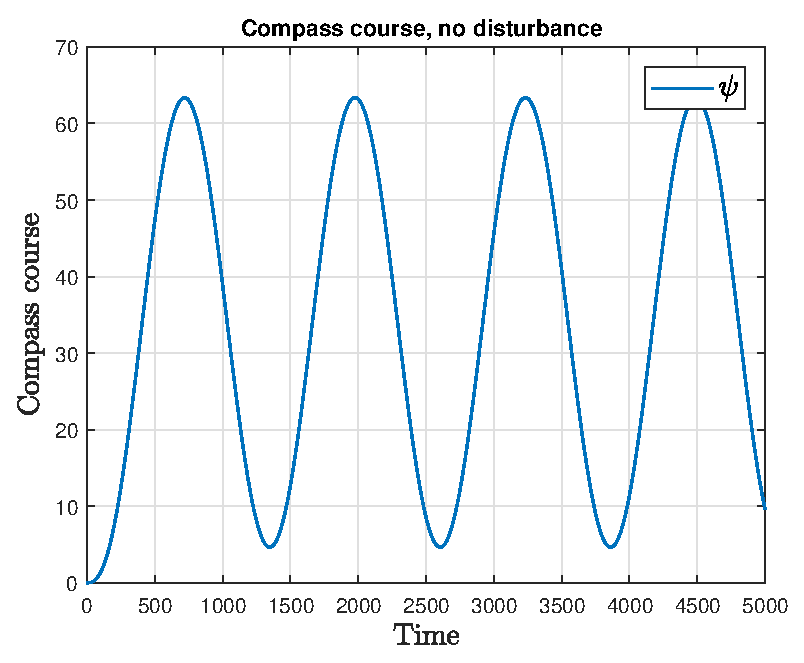
\includegraphics[width = 0.8\textwidth]{figures/plots/P5p1b_heading_005.eps}
    \caption{Compass course response. Rudder input is sine with the frequency of $\omega_1$}
    \label{fig:p1pb_heading_005}
\end{figure}
\begin{figure}
    \centering
    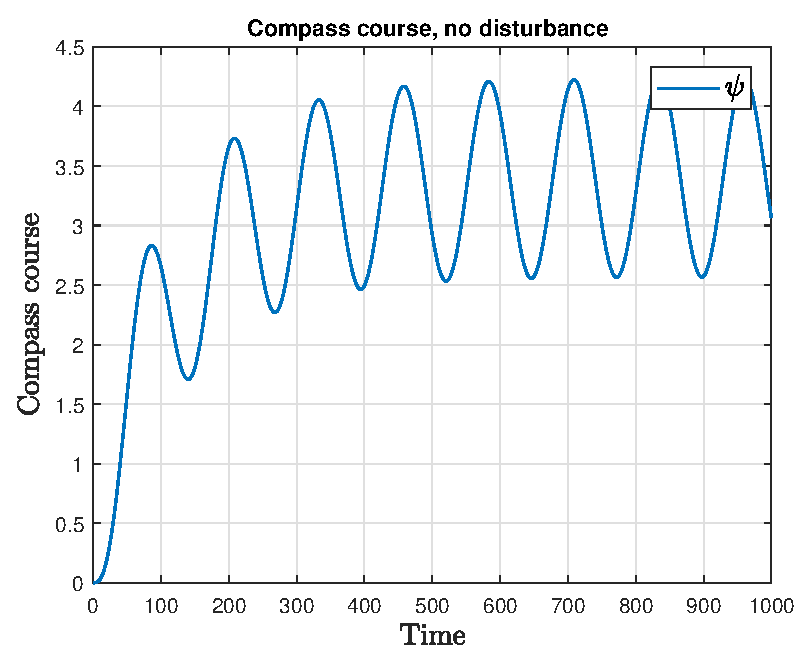
\includegraphics[width = 0.8\textwidth]{figures/plots/P5p1b_heading_05.eps}
    \caption{Compass course response. Rudder input is sine with the frequency of $\omega_2$}
    \label{fig:p1pb_heading_05}
\end{figure}
and measure the amplitudes as seen in \cref{fig:p1pb_heading_005} and \cref{fig:p1pb_heading_05}.  
\begin{align*}
    \abs{H(j\omega_1)} = A_1 = 29.35\\
    \abs{H(j\omega_2)} = A_2 = 0.838
\end{align*}
where $A_1$ and $A_2$ are the amplitudes of the transfer function at $\omega_1$ and $\omega_2$.
By solving the transfer function for $K$ we get
\begin{align*}
    \abs{H(j\omega_1)} &= A_1\\
    \abs{\frac{K}{j\omega_1(Tj\omega_1+1)}} &= A_1\\
    \frac{K}{\abs{j\omega_1(Tj\omega_1+1)}} &= A_1\\
    \frac{K}{\abs{(-T\omega_1^2+j\omega_1)}} &= A_1\\
    \frac{K}{\abs{(-T\omega_1^2+j\omega_1)}} &= A_1\\
    K &= A_1\sqrt{T^2\omega_1^4+\omega_1^2}\\
    K &= A_1\omega_1\sqrt{T^2\omega_1^2+1}\\
\end{align*}
Inserting for $K$ and solving for $T$ we get
\begin{align*}
    \abs{H(j\omega_2)} &= A_2\\
    \abs{\frac{K}{j\omega_2(Tj\omega_2+1)}} &= A_2\\
    \frac{K}{\abs{(-T\omega_2^2+j\omega_2)}} &= A_2\\
    A_1\omega_1\sqrt{T^2\omega_1^2+1} &= A_2 \omega_2\sqrt{T^2\omega_2^2+1}\\
    A_1^2\omega_1^2(T^2\omega_1^2+1) &= A_2^2\omega_2^2(T^2\omega_2^2+1)\\
    (A_1^2\omega_1^4-A_2^2\omega_2^4)T^2 &= A_2^2\omega_2^2-A_1^2\omega_1^2\\
    T &= \sqrt{\frac{A_2^2\omega_2^2-A_1^2\omega_1^2}{A_1^2\omega_1^4-A_2^2\omega_2^4}}\\
\end{align*}
Thus, inserting numerical values, we get that
\begin{align}
    K &= 0.1559 \\ 
    T &= 71.6865
\end{align}

\subsection{C, Estimating with waves measurement noise}
Now we are to repeat the procedure of calculating $T$ and $K$, but now in rough water conditions, with wave and current disturbance turned on. 
Setting the measurement cursors at the peak without noise. 
Repeating the procedure we get 
\begin{align}
    K = 0.3572\\
    T = 444.6904
\end{align}
When trying to estimate the model parameters in rough weather conditions, mainly when we apply an input with the frequency $\omega_2 = 0.05$ it is very hard to distinguish the signal from the wave disturbance as we can see in \cref{fig:p1c_heading_05}. When the system has an input with the frequency of $\omega_1 = 0.005$ it is much easier to distinguish the signal from the wave disturbance. Thus the resulting parameters don't match up with the estimated estimated parameters in calm waters and must be considered useless.
\begin{figure}
    \centering
    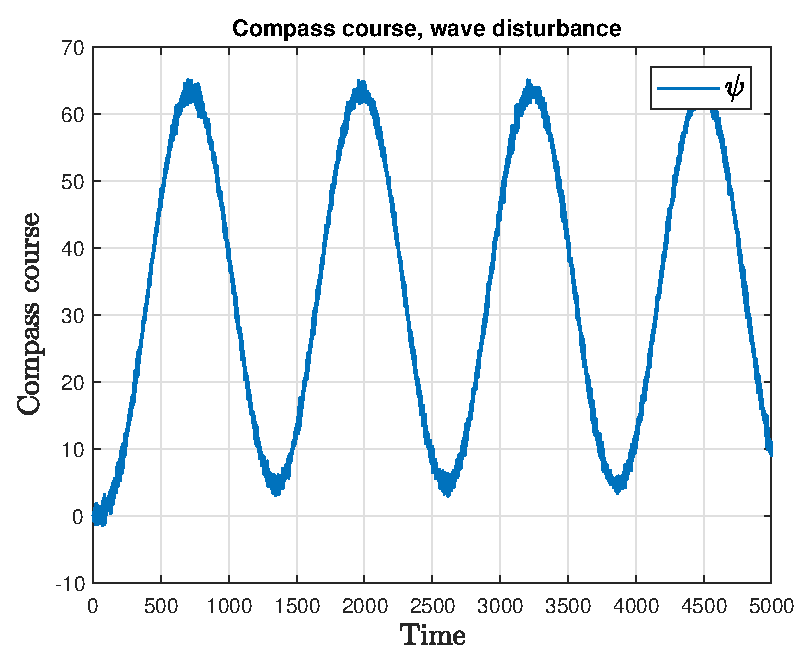
\includegraphics[width = 1.00\textwidth]{figures/plots/P5p1c_heading_005.eps}
    \caption{Compass course response, with wave and current disturbance.  Rudder input is sine with frequency of $\omega_1$}
    \label{fig:p1c_heading_005}
\end{figure}
\begin{figure}
    \centering
    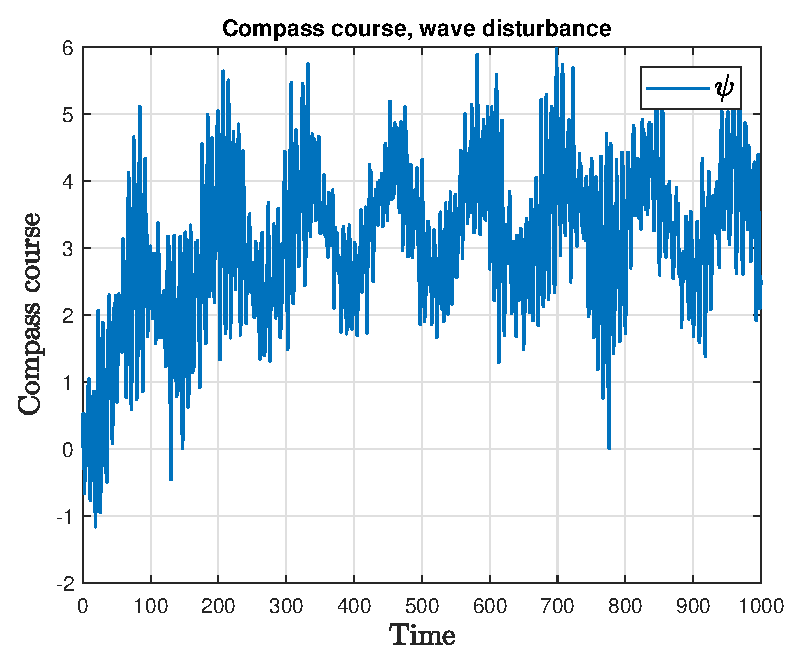
\includegraphics[width = 1.00\textwidth]{figures/plots/P5p1c_heading_05.eps}
    \caption{Compass course response, with waves and current disturbance.  Rudder input is sine with frequency of $\omega_2$}
    \label{fig:p1c_heading_05}
\end{figure}
\subsection{D, Comparing the estimated model to the ship}
We apply a step of rudder angle on the ship model \cref{eq:Transfer_function} as well a a step on the full system model in Simulink.  The step is of one degree. 
The responses are plotted and compared in \Cref{fig:Step response of ship vs ship model}. 
To begin with the model is pretty accurate, but as time goes the model starts to deviate from the response of the ship. For our use the model is a good enough approximation since its most important that the model holds for small values of time. If we did need a more accurate model we could model the physical system in more detail.
\begin{figure}
    \centering
    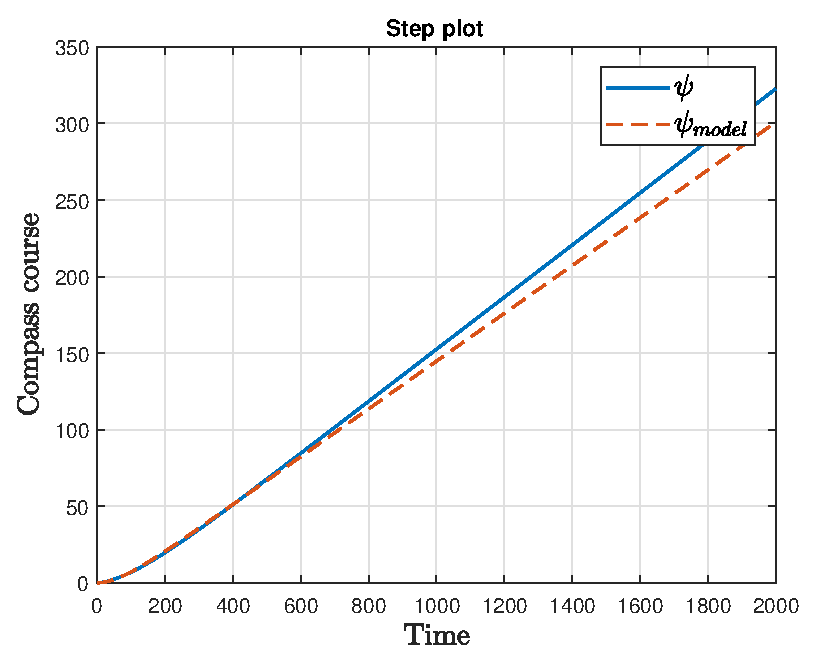
\includegraphics[width = 1.00\textwidth]{figures/plots/P5p1d_heading.eps}
    \caption{Step response of the ship and the ship model.}
    \label{fig:Step response of ship vs ship model}
\end{figure}